% !TEX root = ../my-thesis.tex
%




\chapter{Attack evaluation}
In this chapter we will quantify the effectiveness of our attack. We will begin by explaining our assumptions and evaluation strategy in section \ref{sec:attackeval:prelim}. In section \ref{sec:simresults} we will then present our results for Dilithium, qTESLA and BLISS respectively.  

\section{Preliminaries}
\label{sec:attackeval:prelim}
In this section we will discuss on what assumptions we base our simulations and what kind of parameters we will evaluate. 
\subsection{Assumptions}
\label{sec:simassumptions}
We assume an attacker as described in section \ref{sec:attackmodelgeneral}.
Further will always assume that we as the attacker will have at least as much information as would be sufficient to break the signature scheme if the shuffling countermeasure would not be used. This translates to the fact that we will always have $n$ or more faulted coefficients which correspond to at least $n$ linear independent equations. This is because without the shuffling countermeasure an attacker would know which coefficients were faulted (the last few), take the corresponding linear equations and solve them using gaussian elimination.



\subsection{Notion of success}
\label{sec:simsuccess}
For a certain $m$ we will say that we were successful in breaking the signature scheme, if we manage to succeed recovering the entire secret in at least two out of three tries, i.e. we have a success rate of at least around $66\%$. Each try fails after a timeout of 5 minutes wall time.

\subsection{Parameter evaluation}
When we use only the minimal mount of signatures required to fulfill our aforementioned requirements the attack will not show optimal results.
Thus, for Dilithium, we will evaluate two parameters of our attack which we hope to improve our results:
\begin{enumerate}
	\item surplus of equations $p$
	\item threshold $t$
\end{enumerate}
For qTESLA and BLISS we will only evaluate the parameter $p$. 

The surplus of equations $p$ is the minimal amount of additional faulted equations, relative to the minimum described in  \ref{sec:simsuccess}.
In our simulations we control this value by generating signatures until we can guarantee that we have has at least $n + p$ faulted equations out of which where exist $n$ linear independent ones. Note that using this approach the resulting amount of faulted equations may be higher than the surplus of equations parameter, because a single signature might produce more than one faulted signature.

The threshold parameter is used as to steer the false-positive rate as described in detail in section \ref{sec:prefilter}. The lower the threshold, the lower the false-positive rate and vice versa.
The false-positive rate is dependent on both, $m$ and $t$. Thus for a fixed $m$ the false-positive rate only depends on $t$.

We choose the two parameters based on the following two arguments:

We argue that a greater surplus of equations opens more choices to the ILP-solver to classify enough equations properly and thus the searchspace will more likely contain an easy-to-find path to a solution.
The arguing with the false-positive rate is that a lower false-positive rate makes (random) positive classification guesses of the ILP-solver more likely to be correct and thus the ILP-solver should reach its objective quicker, eventually recovering the secret polynomial. Additionally a lower false-positive rate reduces the total amount of equations required to have at least $n$ true equations. This reduces the amount of total variables and thus the difficulty of the generated ILP instance.


We tested our hypothesis statistically by running attack simulations for Dilithium (NIST security level II) for $f = 1, \ldots 10$. Recall that $f$ denotes the amount of faulted coefficients. We do not choose higher $f$ because we empirically know our attack almost always succeeds in that case.



\begin{figure}%
		\centering%
		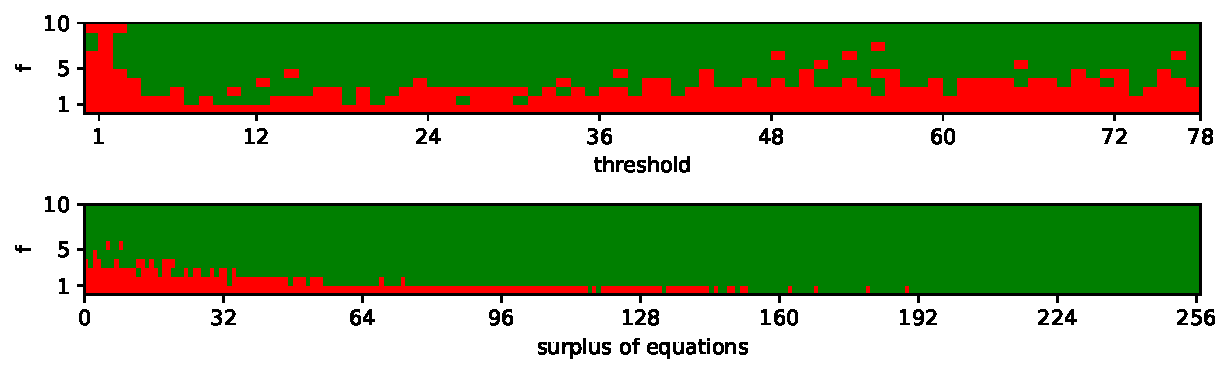
\includegraphics[width=.95\linewidth]{plots/threshold_pccolormesh}%
		%\caption{threshold ($s$)}%
	\caption{Heatmap showing the correlation between threshold and success as well as the correlation between surplus and success for $f = 1, \ldots,10$. A red rectangle indicated a failed attack, a green rectangle indicated a successful attack.}
	\label{fig:heatmap}%
\end{figure}

The heatmap \ref{fig:heatmap} clearly shows that the surplus parameter has an effect on the attack performance which is also confirmed by the Pearson correlation coefficients in Figure \ref{fig:corrs}.
For the threshold parameter on the other hand this is not directly clear. Our data shows that the attack performance is poor when extremely low thresholds are used. We think that an extremely low threshold affects a parameter other than the false-positive rate and this to us unknown parameter has a negative impact on the attack performance.
This phenomena can also be seen in Figure \ref{fig:corrthreshold}: For $f \geq 6$, we see a positive correlation is caused by the poor attack performance with for extremely low thresholds. For smaller $f$ we see a negative correlation, due to the low  false-positive rate. While the absolute value of the correlation coefficient for $f \leq 5$  is not very big, taking into consideration that it also has to compensate for the poor performance when the threshold is extremely low, the positive effect of the threshold to the attack performance is not neglectable.

\begin{figure}%
	\centering%
	\begin{subfigure}{.5\textwidth}%
		\centering%
		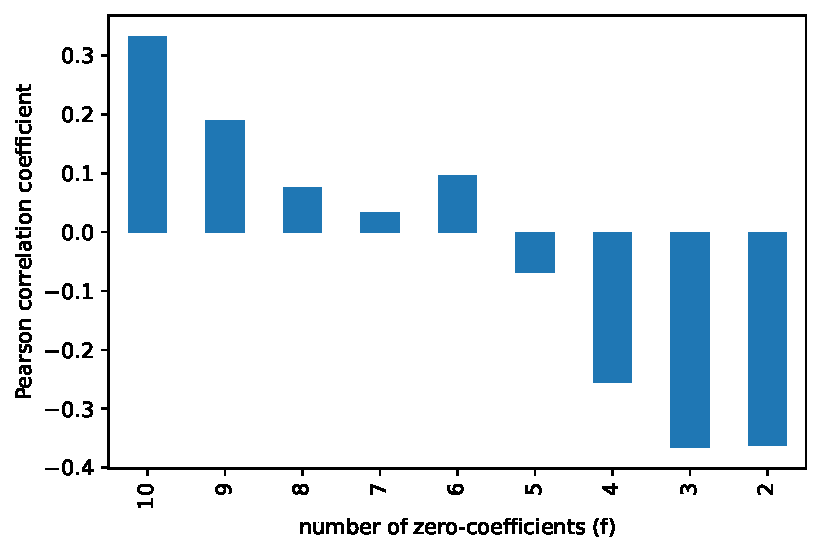
\includegraphics[width=.95\linewidth]{plots/threshold_correlation}%
		\caption{threshold $t$}%
		\label{fig:corrthreshold}%
	\end{subfigure}%
	\begin{subfigure}{.5\textwidth}%
		\centering%
		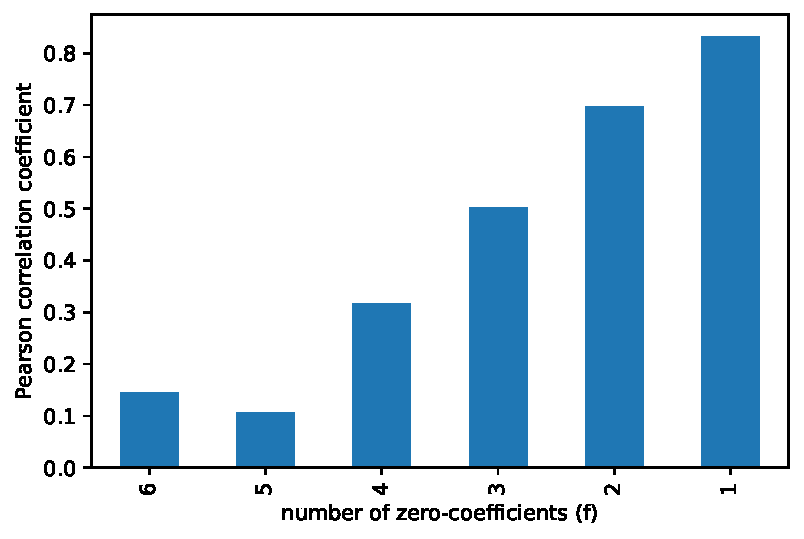
\includegraphics[width=.95\linewidth]{plots/surplus_correlation}%
		\caption{surplus of equations $s$.}%
		\label{fig:corrsurplus}%
	\end{subfigure}%
%
	\caption{The minimal required surplus of equations and the corresponding signature count per $f$. If a bar is not present it means that no surplus was required for that security level and $f$.}
	\label{fig:corrs}%
\end{figure}




When we perform an attack with default parameters, we mean we will use a threshold which does not filter any true-positive equations, we fulfill the assumptions defined in section \ref{sec:simsuccess} and all that with the minimal amount of signatures required.



\subsection{Parameter evaluation strategy}
In general the simulations aim to find out how lax we can be in the timing of the fault, which translate to how high we can go with the iteration number $m$, after which we will induce a fault. While in the simulations we will fault exactly $f$ coefficients per signature, the simlation results can be translated to an attacker who faults on average $f$ coefficients per signature.




    \begin{algorithm}
        \SetKwFunction{print}{print}
        $t \gets \beta$ \tcp{threshold}
        $f \gets nl$ \tcp{number of zero-coefficients; $m = nl - f$}
        \While{$f \geq 1$ and $t \geq 1$}{
            \eIf{at least $2$ out of $3$ attacks successful}{
                \print{for $f$ zero-coefficients we need a threshold of no more than $t$}\;
                $f \gets f - 1$\;
            }{
                $t \gets t - 1$\;
            }
        }
        
        \caption{Evaluation strategy for the $s$ parameter.}
        \label{alg:surplus}
    \end{algorithm}
    
    %\phantom{hi}
    \vspace{4em}
    
    \begin{algorithm}
        \SetKwFunction{print}{print}
        $s \gets n$ \tcp{surplus}
        $f \gets nl$ \tcp{number of zero-coefficients; $m = nl - f$}
        \While{$f \leq 1$ and $s \leq 2n$}{
            \eIf{at least $2$ out of $3$ attacks successful}{
                \print{for $f$ zero-coefficients we need a surplus of at least $s$}\;
                $f \gets f - 1$\;
            }{
                $s \gets s + 1$\;
            }
        }
        
        \caption{Evaluation strategy for the $t$ parameter.}
        \label{alg:threshold}
    \end{algorithm}






%The parameters $p$ % and $t$
%will be evaluated as follows: We start with $m_0 = s_0 = 0$ and as long as our attack succeeds we increment $m$ by one and continue our simulations. When we reach a $m$ where we do not succeed with our current $s$ we will repeat the simulation for the same $m$ but an incremented $s'$, which is calculated as the previous amount of faulted equations incremented by $1$. Note that the previous amount of faulted equations may be higher than $s$, as $s$ is defined a minimum. When we reach a $s$ where our attack succeeds we again continue to only incrementing $m$ until again our attack does not succeed anymore and we repeat the strategy.

%When evaluating the parameter $t$ we will start with $m = 0$ and a $t$ which does not filter any true-positive equations. We increment $m$ until our the attack fails. If that is the case we decrement $t$ by one and try again for that $m$ until we succeed. Once we reached a $t$ where we succeed we again begin to increment only $m$ until again our attack does not succeed anymore and we repeat the strategy.

The evaluation strategy for the parameter \say{surplus of equations} and \say{threshold} are depicted in Algorithm \ref{alg:surplus} and \ref{alg:threshold} respectively.
Using these strategies we will be able to determine for every $m$ if our attack succeeds, and if yes, what parameter value is necessary for success.

\subsection{Simulation hard- and software}
\label{sec:practise_server}
The ILP-solver used for our simulations is Gurobi \footnote{\url{https://www.gurobi.com/}}.
Our simulation is written in Python using the Numpy library \footnote{\url{https://numpy.org/}} and the gurobipy library \footnote{\url{https://pypi.org/project/gurobipy/}} for the Gurobi Python bindings. All simulations were run on a computer with a Intel\textsuperscript{\textregistered} Xeon\textsuperscript{\textregistered} Processor E7-4870 (4 sockets, 10 cores, using 40 out of 80 available threads @ 2.4GHz) with 500GB of RAM.


\section{Simulation results}
\label{sec:simresults}
In this section we will discuss the results of our simulations. First we will start with a thorough discussion on the results for Dilithium, as we will evaluate and compare both the parameters $s$ and $p$. Next we will follow with qTESLA as well as BLISS. In the end we will discuss how the repetition rate affects the required amount of signatures.

\subsection{Dilithium}
For Dilithium we will first discuss the results when our default parameters are used. Then we will discuss the results for both, the parameter $s$ and the parameter $t$. Finally we will compare the results of both parameters.

\subsubsection{Default parameters}
\label{sec:min_sig_amount}

\begin{figure}
	\centering
	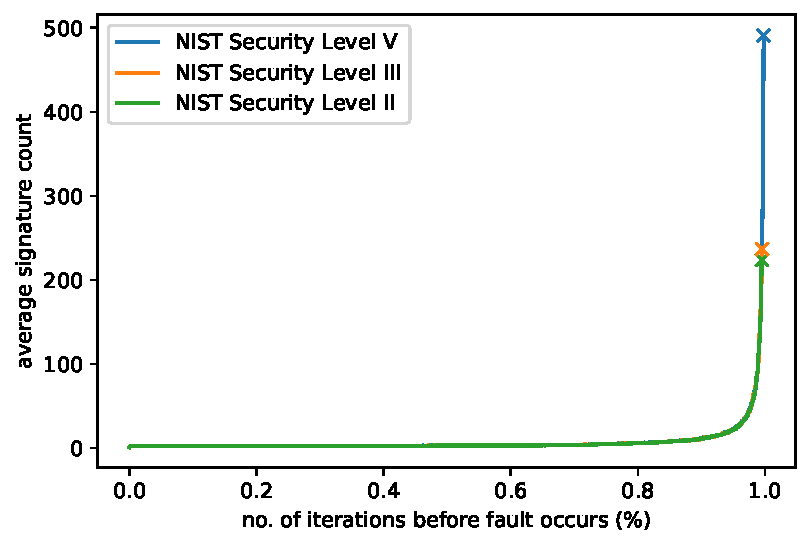
\includegraphics[width=.7\linewidth]{plots/dilithium_sigcount_noparams}
	\caption{Average amount of signature required for a successful attack per $m$ in percent (relative to $nl$). The amount of signatures is very similar throughout all security levels for early iteration aborts. Thus the green line covers the other two. Crosses indicate the maximum signature count.}
	\label{fig:dilithiumsigcountnoparams}
\end{figure} 

When using the default threshold described in section \ref{sec:prefilter} and a surplus of $0$ our attack succeeds for $f$ as low as $5$, $6$ and $4$ requiring $224$, $236.5$ and $491$ signatures on average for the NIST security levels II, III and V respectively.
Further we observe that the higher the NIST security level the more signatures are required. This is due to the fact that minimum amount of equations increases as the security level increases  because the parameter $l$ increases for every security level.  Recall that the minimum amount of required equations is $nl$ for Dilithium. The amount of signatures required per $m$ is depicted in Figure \ref{fig:dilithiumsigcountnoparams}.

\subsubsection{Surplus of equations}
\label{sec:dilithiumsurplus}

\begin{figure}%
	\centering%
	\begin{subfigure}{.5\textwidth}%
		\centering%
		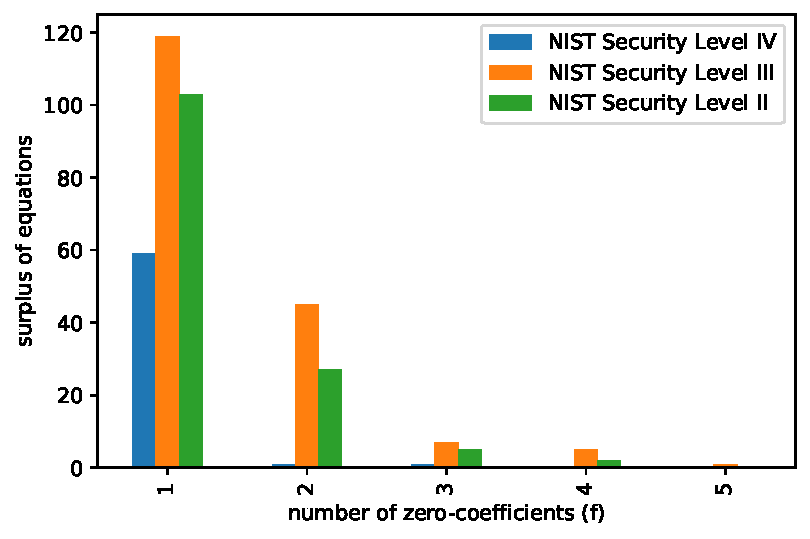
\includegraphics[width=.95\linewidth]{plots/dilithium_surplus}%
		\caption{Surplus of equations per $f$}%
		\label{fig:dilithiumsurplus}%
	\end{subfigure}%
	\begin{subfigure}{.5\textwidth}%
		\centering%
		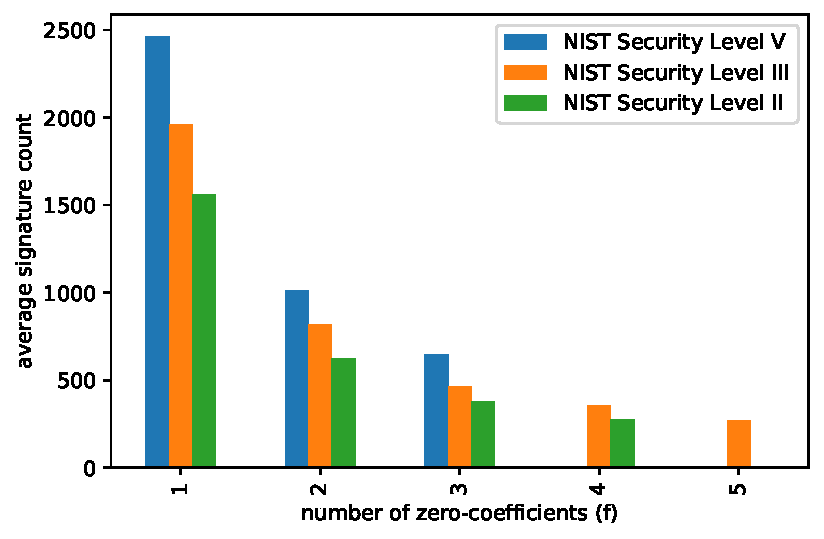
\includegraphics[width=.95\linewidth]{plots/dilithium_sigcount_upper}%
		\caption{Corresponding signature count per $f$.}%
		\label{fig:dilithiumsigcountsurplus}%
	\end{subfigure}%
%
	\caption{The minimal required surplus of equations and the corresponding signature count per $f$. If a bar is not present it means that no surplus was required for that security level and $f$.}
	\label{fig:dilithiumsigcountsurplussurplus}%
\end{figure}

Our simulation results show, that for every $m$, we are able to succeed our attack.
This means that an attacker who is able to (on average) fault a single coefficient of $\bm{y}$ can recover $\bm{s}_{1}$, given that he can do it on around $1562$,  $1959.5$, $2465$ signatures for NIST security level II, III and V respectively. The surplus of equations required per $m$ as well as the amount of signatures required per $m$ are depicted in Figure \ref{fig:dilithiumsigcountsurplussurplus}.

We can observe that the signature count increases as $f$ decreases, as well as when the security level increases. First is due to the fact that we get less zero-coefficients per signature and letter is the case because higher security levels require more zero-coefficients in total ($nl$ many) as $l$ increases as the security level does.



\subsubsection{Threshold}
\label{sec:evalthreshold}

\begin{figure}%
	\centering%
	\begin{subfigure}{.5\textwidth}%
		\centering%
		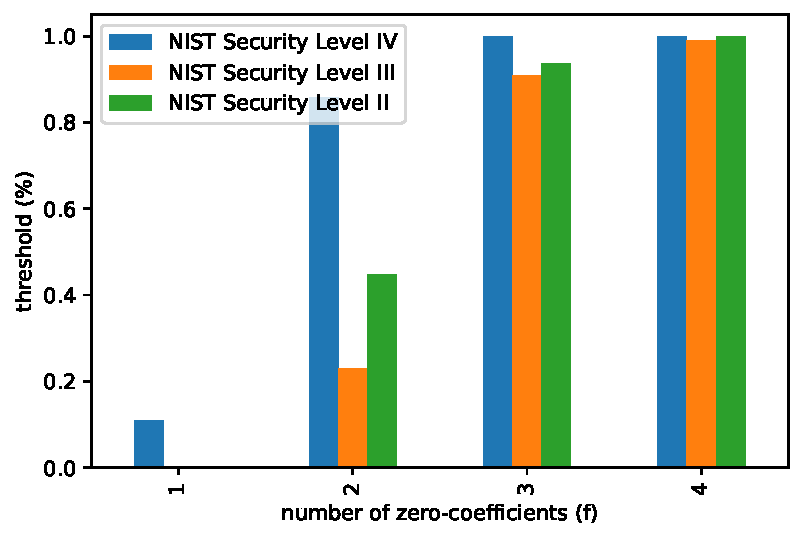
\includegraphics[width=.95\linewidth]{plots/dilithium_threshold_percent}%
		\caption{Maximum possible threshold ($\%$).}%
		\label{fig:dilithiumthreshold}%
	\end{subfigure}%
	\begin{subfigure}{.5\textwidth}%
		\centering%
		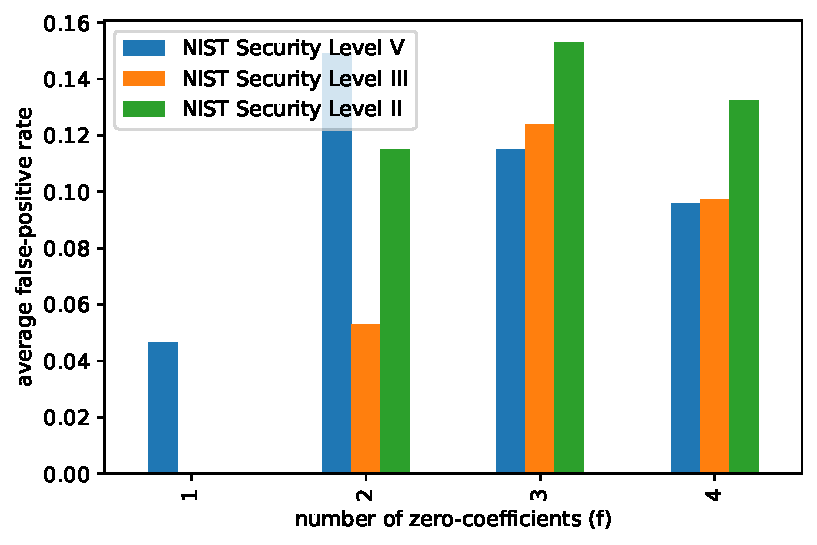
\includegraphics[width=.95\linewidth]{plots/dilithium_threshold_fpr}%
		\caption{Corresponding false-positive rate.\phantom{}}%
		\label{fig:dilithiumthresholdfpr}%
	\end{subfigure}\\\vspace{1em}%
	\begin{subfigure}{.5\textwidth}%
		\centering%
		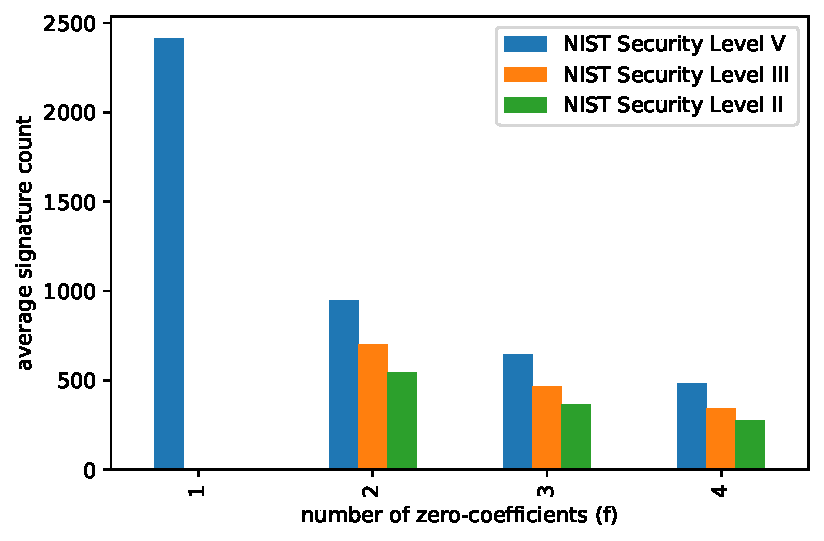
\includegraphics[width=.95\linewidth]{plots/dilithium_threshold_sigcount}%
		\caption{Corresponding signature count.}%
		\label{fig:dilithiumthresholdsigcount}%
	\end{subfigure}%
%
	\caption{The maximum possible threshold per $f$ and the corresponding false-positive rate as well as the corresponding signature count.}
	\label{fig:dilithiumthresholdall}%
\end{figure}
We evaluated the threshold parameter for $f \leq 4$ as for higher $f$ our attack succeeded without needing a reduced threshold.
We were able to succeed our attack for all $f \geq 2$ for all NIST security levels. With a single coefficient faulted our attack succeeded only for security level V.

In Figure \ref{fig:dilithiumthreshold} we observe that as $f$ decreases ($m$ increases) we require a lower threshold to succeed. This can be explained because as $f$ decreases for a fixed threshold we will have an increased false-positive rate. To achieve the same or lower false-positive rate as we had with $f + 1$ we require a lower threshold. 

Comparing the threshold of different security levels for a fixed $f$ is difficult because the distributions of $c\bm{s}_1$ differs for different the security levels. This kind comparison is better performed by looking at the false positive rate. 

%If we compare the relative threshold for fixed $f$ but different security levels we notice that the relative thresholds are similar for $f = 3, 4$, but very different for $f = 1$. Latter we can not properly explain. It might be due to lucky/unlucky ILP instances.

Inspecting the false-positive rate in Figure \ref{fig:dilithiumthresholdfpr} for $f=3, 4$ we observe that the higher the security level the lower the false-positive rate. This behavior is expected as $l$ ILPs need to be solved per attack and $l$ increases as the security level increases. As all security levels have the same time limitation, higher security levels need to solve more ILPs per fixed time and thus have less time per ILP. To solve an ILP in a shorter timeframe the attacker requires easier ILP instances. Thus a lower false-positive rate is required. %Finally again we can not properly explain the data for $f=1$.

For $f = 2$ and security level V we are unable to properly explain the suddenly increasing false-positive rate. It might be that by chance, despite the high false-positive rate, the ILP instances were easy.

The signature count (Figure \ref{fig:dilithiumthresholdsigcount}) increases as $f$ decreases and also for a fixed $f$ the signature count increases as the security level does.
Both of these phenomena have been explain in the previous section \ref{sec:dilithiumsurplus}.

\subsubsection{Comparison}
\label{sec:dilithiumcompare}
Looking at the aspect of for which $f$ we are able to perform a successful attack we can see that when using the \say{surplus of equations} parameter we can do so for any $f$ and any security level, whereas using the \say{threshold} parameter we are only able to do so for for all $f \geq 2$ and $f = 1$ only for security level V. 
The amount of signatures required is similar for both parameters.
%When comparing the amount of signatures which are needed for a successful attack per $f$ we  observe that when using the \say{surplus of equations} parameter we need slightly more signatures to succeed than with \say{threshold}.

%We value the fact that we are able to succeed with a higher $m$ more than the slightly decreased signature amount.
Thus we conclude that the parameter \say{surplus of equations} has a bigger impact on the attack performance than \say{threshold}.
Albeit we note that both parameters have impact on the attack performance. While the optimal solution is probably to use both parameters together with a certain weight, the attack results of the \say{surplus of equations} parameter are good enough for our use-case so that we will not do further research to increase the performance.
Additionally, because the attack strategy is very similar for the other two signature schemes, we believe that the results we obtained for Dilithium can also be applied to the other two signature schemes. Thus we will only evaluate the \say{notion of success} parameter for qTESLA and BLISS.

\subsection{qTESLA}

\begin{figure}[p]
\centering
\begin{subfigure}{.5\textwidth}
  \centering
  
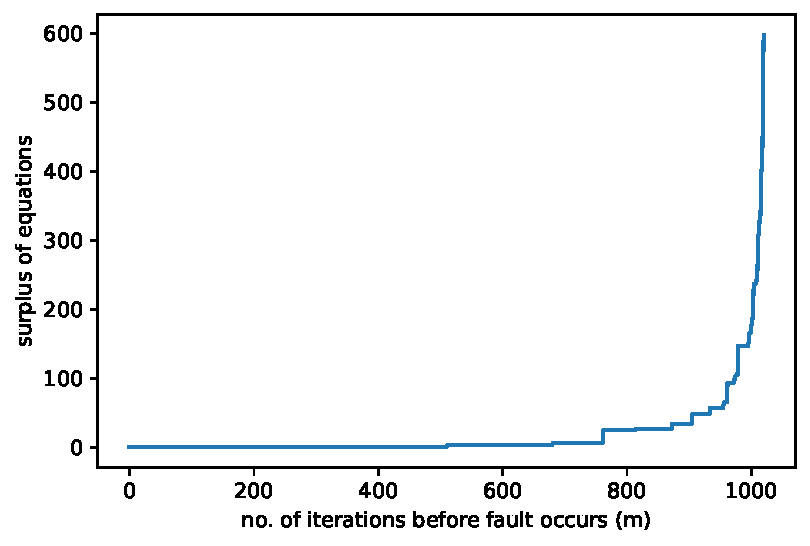
\includegraphics[width=.9\linewidth]{plots/server_qtesla_i_surplus}%
  \caption{Surplus of equations per $m$.}
  \label{fig:resqteslasurplus}
\end{subfigure}%
\begin{subfigure}{.5\textwidth}
  \centering
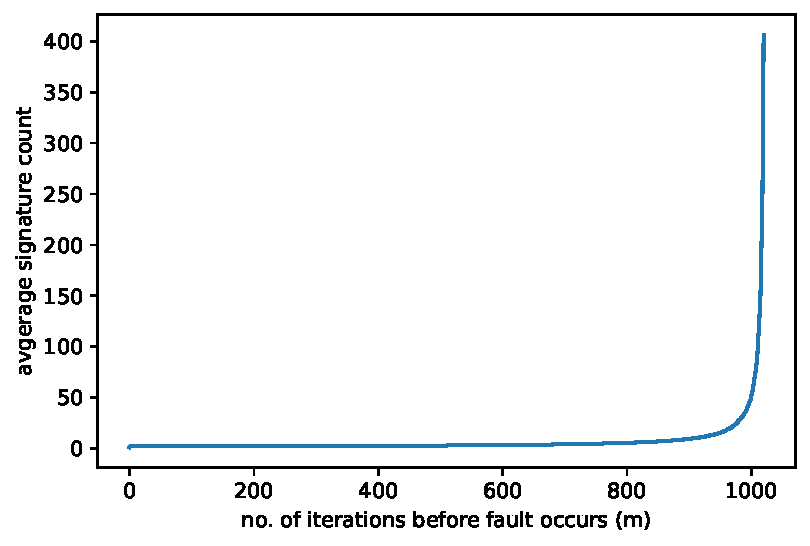
\includegraphics[width=.9\linewidth]{plots/server_qtesla_i_sigcount_surplus}%
  \caption{Corresponding signature count per $m$.}
  \label{fig:resqteslasigs}
\end{subfigure}

\caption{qTESLA (NIST security level I) simulation results. The minimal required surplus of equations and the corresponding signature count per $m$.}
\label{fig:resqtesla}
\end{figure}



%When evaluating the parameter we choose to increase it by 10 whenever the attack fails. We do this because in depending on the parameter set qTESLA's $n$ is 4 or 8 times as large as in Dilithium's and thus the increase of the parameter relative to $n$ is smaller. To finish our simulations in a reasonable amount of time we therefore increase the step size.

Our simulation results show that we are able to break the shuffling countermeasure for the parameter set \texttt{qTESLA-p-I} (NIST security level I) but not so for the parameter set  \texttt{qTESLA-p-III}  (NIST security level III) for any reasonable $m$.
When attacking security level I using the default parameters our attack succeeds for all $m \leq 510$. Using the \say{surplus if equations} parameter we were able to succeed with only two faulted coefficients for which we require on average of $406$ signatures. The exact results for security level I can be found in Figure \ref{fig:resqtesla}.
 
Compared to Dilithium and BLISS qTesla works on a way higher dimension even in the NIST security level I ($n = 1024$). Thus we assume this is the reason we were unable to break NIST security level III of qTESLA, as it doubles the dimension compared to security level I to $n = 2048$. Higher dimensions result in higher variable-count in the corresponding ILP, exponentially increasing the difficulty to solve it.

\subsection{BLISS}

\begin{figure}%
	\centering%
	\begin{subfigure}{.5\textwidth}%
		\centering%
		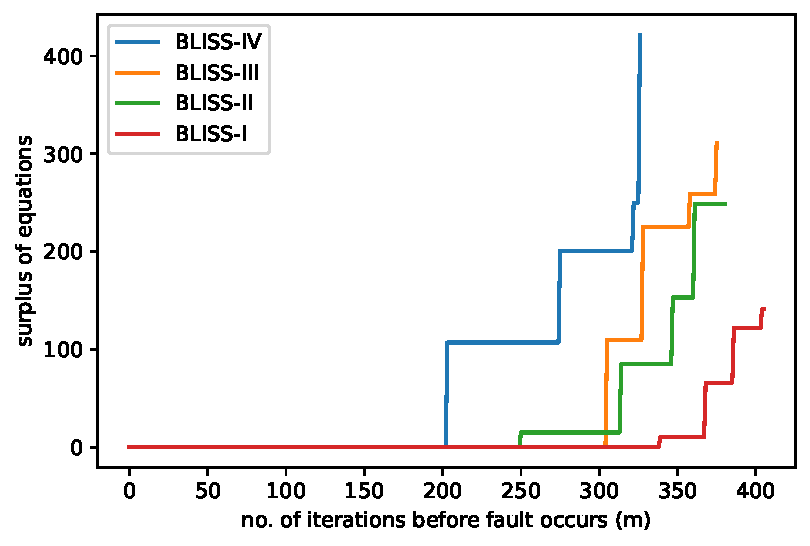
\includegraphics[width=.95\linewidth]{plots/bliss_surplus}%
		\caption{Surplus of equations per $m$.}%
		\label{fig:blisssurplus}%
	\end{subfigure}%
	\begin{subfigure}{.5\textwidth}%
		\centering%
		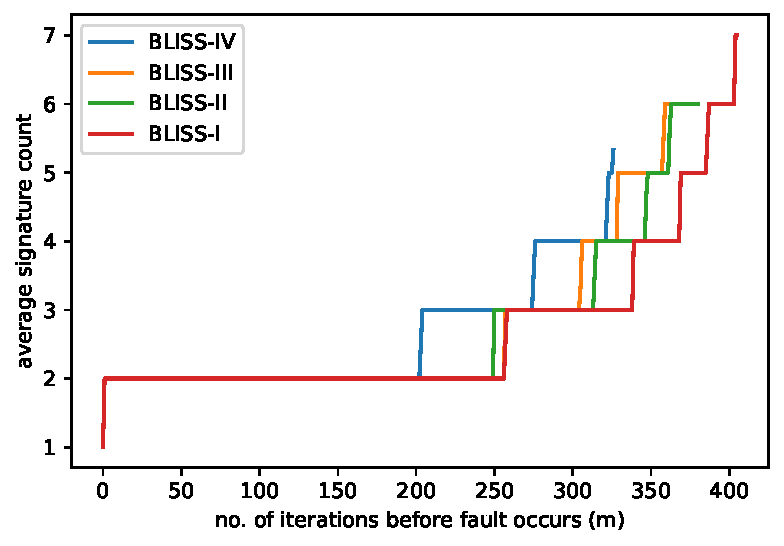
\includegraphics[width=.95\linewidth]{plots/bliss_surplus_sigcount}%
		\caption{Corresponding signature count per $m$.}%
		\label{fig:blisssurplussigcount}%
	\end{subfigure}%
%
	\caption{BLISS simulation results. The minimal required surplus of equations and the corresponding signature count per $m$.}
	\label{fig:blisssurplusandsigcount}%
\end{figure}


The authors of BLISS propose four different parameter sets, BLISS-I, BLISS-II, BLISS-III and BLISS-IV which aim to offer 128, 128, 160 and 192 bits of security respectively \cite[pp.~23--24]{bliss_full}. We were able to successfully attack all these parameter sets, though in contrast to Dilithium and qTESLA (NIST security level I) % and qTesla (\texttt{qTESLA-p-I})
we require the loop-abort to be more early. To be precise the loop-abort needs to occur at least prior the $405$th loop iteration, which is  around $80\%$ of the total iteration count.

The surplus of equations needed per $m$ and the corresponding required amount of signatures are depicted in Figure \ref{fig:blisssurplusandsigcount} for all BLISS parameter sets.



\subsection{Repetition rate and required amount of signatures}


All the schemes we attack are based on the Fiat-Shamir with aborts design. Thus these schemes may abort and retry. The expected amount of tries before the schemes output a valid signature is called the repetition rate. An attacker can not a priori know the repetition rate, thus he can not perfectly time his fault a priori. 

If the attacker model is strong enough such that an attacker can induce multiple loop abort faults during the signature generation, one for every possible repetition, the amount of signature required matches with the numbers we present here. If the attacker model is less strong, such that the fault can only be executed for one specific repetition count, e.g. only the first repetition, then the amount of signature required will increase, depending on the signature scheme and parameter set.

For deterministic signature schemes like Dilithium an attacker can generate a signature of a message $μ$ without fault and observe the repetition rate by time measurements. Using this repetition rate he can set a proper timing for the fault (loop abort in the last repetition) and sign $μ$ again, but this time with the a fault induced in the last repetition. Such an approach would double the amount of signature generations which need to be performed.

This does not work for probabilistic signature schemes, like BLISS and qTESLA. In this case an attacker has to set up the timing for a fault in the first repetition and repeat the signature generation until a signature is outputted after the first try. In this case the amount of signatures needed has to be scaled by the repetition rate of the particular scheme and parameter set.

qTESLA NIST security level I has an acceptance rate of $.13$ \cite[p.~452]{qtesla}, thus a repetition rate of  $7,69$. The amount of required signatures need to be scaled by $7,69$.
The repetition rates for Dilithium and BLISS can be found in Table \ref{table:dilithium} and \ref{table:bliss} respectively.

Finally we want to highlight that the repetition rate does not, other than the required signatures, affect our attack efficiency, e.g. difficulty of ILP instances or the false-positive rate. The repetitions performed for a particular signature can be detected by time measurements and thus signatures which did not match the expected repetition rate will be discarded and never appear in the actual attack data.



\begin{table}
\centering
\begin{tabular}{ c c c c }
 NIST Security Level & II & III & V \\ 
 \hline
 Repetition rate & $4.25$ & $5.1$ & $3.85$ \\  
\end{tabular}\vspace{1em}
\caption{Repetition rates for the Dilithium signature scheme \cite[p.~16]{dilithium_spec}.}
\label{table:dilithium}
\end{table}

\begin{table}
\centering
\begin{tabular}{ c c c c c }
 Parameter set & BLISS-I & BLISS-II & BLISS-III & BLISS-IV \\ 
 \hline
 Repetition rate & $1.6$ & $7.4$ & $2.8$ & $5.2$ \\  
\end{tabular}\vspace{1em}
\caption{Repetition rates for the BLISS signature scheme \cite[p.~24]{bliss_full}.}
\label{table:bliss}
\end{table}
